\documentclass{../src/bcthesispart}
\title{Emerging numeral systems}
\author{Bas Cornelissen}
\begin{document}

%——————————————————————————————————————————————————————————
\parttitle{Emergent numeral systems}%
	{Emergent numeral systems}
	{counting-games}{%
	% Abstract
	% --------
	Numeral systems seem to be an ideal testbed for models of language evolution.
	They have a clear hierarchical, recursive structure, there is plenty of variation, and their structure suggests how they evolved.
	So what can the models of language evolution discussed in the first part of this thesis tell about the emergence of numeral systems?
	This chapter addresses that question.
	To that end we first revisit and reinterpret the work of James Hurford, who addressed the same question over 30 years ago.
	This reveals that naming games can be sensitive to biases in the domain, which can be distinguished from biases of the agents. 
	Finally, an attempt to simulate the evolution of numeral systems directly is presented and discussed.
	}
%——————————————————————————————————————————————————————————





\noindent
Numeral systems strongly restrict the set of allowed expressions for numbers.
One would be surprised to find a book for \emph{three fours and seven euros} — that number is called \emph{nineteen}. 
The degree of standardisation, to put it differently, is remarkably high for numerals.
Why so?
\textcite{Hurford1987} wonders whether the standardisation could be the result of a process of social interaction.
In his  account of the evolution of numeral systems, linguistic innovators play an important role.
These rare individuals occasionally invent new linguistic constructions, such as additive or multiplicative constructions.
Between phases of linguistic innovation the invented rules spread the population and do not change substantially, until the next innovation comes along.
This might be an idealisation, but even if one prefers gradual phases of innovation rather than an individual innovator, the question remains how a linguistic innovation eventually become standardised.
%%



Hurford addresses the standardisation of a base, the most salient characteristic of a recursive numeral system.
Using two\footnote{%
	%>>>
	Hurford discusses several other variants. I restrict myself to the two  his simulations which appear to be most important for his argument.
	%<<<
	}
agent-based simulations, he argues that the standardisation of a shared base could be the result of a process of social negotiation.
In line with current terminology, I have baptised the simulations the \emph{additive} and \emph{multiplicative Base Game} (\textsc{bg}).
The simulations represent two successive ‘stages’ in evolutionary history, following the invention of additive and multiplicative constructions respectively.
This chapter starts by revisiting Hurford’s work, then moves on to some further simulations and concludes with a discussion.
%%




%——————————————————————————————————————————————————————————
%——————————————————————————————————————————————————————————
\section{Hurford’s base games}
%——————————————————————————————————————————————————————————
%——————————————————————————————————————————————————————————


In both base games, populations of $N$ agents “spend their time uttering numeral expressions to each other”: constructions like $7+6$ or $3\times 10 + 5$.
Interaction between agents are assumed to be homogeneous.
Initially, all agents will use different expressions for the same numbers, but over time the same \emph{base} should be used to form expressions.
Since a base is not defined outside a numeral system, Hurford takes the base to be the largest of the constituents: the base of both $a\times b$ and $a\times b+c$ is $\max(a,b)$.
So $3\times 7, \;\; 4 \times 7 + 3$ and $4+7$ all use base 7. 
Note that the summand $c$ in a multiplicative construction can thus be larger than the base.
We return to these assumptions in the discussion.
%todo discuss: notion of base
%%




Hurford assumes speakers try to use expressions that a hearer is likely to know.
To that end agents track the frequencies or scores $s(b)$ of all bases $b$ they encounter.\footnote{%
	%>>> 
	In this chapter $b$ does not denote the bottleneck, but a base.
	%<<<
	}
A simple criterion decides which bases are \emph{favoured}, i.e.\ which bases an agent prefers to use.
A base $b$ is \emph{favoured} if 
%-
\begin{align}
	\label{eq:favoured-base-criterion}
	%-----
	s(b) > 0 
	\qquad \text{and} \qquad 
	s(b) \ge \xi \cdot \max_{b'} s(b'),
\end{align}
%-
for $1 \ge \xi > 0$.\footnote{%
	%>>>
	Hurford does not require $s(b)>0$, but this simplifies the discussion and does not alter the behaviour of the game.
	%<<<
	}





Just like $\zeta$ in the the Bayesian language games, the parameter $\xi$ determines the production strategy: how much the agent tends towards using the most frequent bases.
For $\xi=1$ the base with positive and maximal frequency are favoured.
The smaller $\xi$ gets, the lower the threshold for being favoured.
This slows down convergence, and I have used $\xi=1$ throughout this chapter. 
Appendix \ref{app:counting-games} includes a brief analysis of the effects of $\xi$.
The set of bases favoured by agent $A$ is denoted $F(A)$.
%%





%——————————————————————————————————————————————————————————
\paragraph{additive base game}

It will be convenient to reformulate Hurford’s models in a more formal fashion.
Suppose agents know simple numerals for the numbers $\mathcal{S} = \{1, \dots, B=2K\}$, which they can combine in additive constructions.
We assume $B = 2K$ to be even as it greatly simplifies the discussion.
Since agents generally prefer to use the simple numerals for numbers below $B$, they only form complex numerals for the numbers $\mathcal{N} = \{ B+1, \dots, B+B \}$, which I call the \emph{domain}.
This implies that the numerals $n \in \mathcal{S}$ for which $n+n < B+1$ cannot be used as a base. 
For example, if $B=10$, agents know simple numerals $\{1, \dots, 10\}$, communicate about the domain $\{11, \dots, 20\}$ using bases in $\{6, \dots, 10\}$.
Note that base 10 is most \emph{expressive} since it can be used to form expressions for all numbers in the domain.
With base 9 you can only get to 18, with 8 up to 16, and so on. 
To make this precise, note that there are $K$ numbers that could be used as a base, namely
%-
\begin{equation}
	b_1 := K+1, \quad b_2 := K+2, \quad \dots \quad b_K := K+K =B
\end{equation}
%-
For the set of numbers $n$ that are \emph{expressible by base $b$} we write
%-
\begin{equation}
	E(b) 
		= \{ n \in \mathcal{N}: n \le b+b \},
\end{equation}
%-
Conversely $E^{-1}(n) = \{b : n \in E(b)\}$ denotes the set of bases that express $n$.
%%




\textcite{Hurford1987} only considered the decimal case $B=10$.
He argued that because 10 is most expressive, it will soon become the most frequent base, resulting in the standardisation of the expressions $10+1, 10+2, \dots, 10+10$.
The additive base game was proposed to test the consistency of this account and follows the following script.
%...
\begin{enumerate}
	\item A number $n\in\mathcal{N}$ is chosen from the domain.

	\item The speaker considers the set $C = F(S) \cap E^{-1}(n)$ of candidate bases: favoured bases that moreover express $n$. She randomly picks a base $b$ from $C$ if it is nonempty, or from $E^{-1}(n)$ otherwise. The speaker expresses $n$ as $b + (n-b)$.
		
	\item The hearer $H$ receives the expression, determines the base used,  and updates the score $s_H(b)$ of $b$ by 1.
\end{enumerate}
%...
%%



\paragraph{multiplicative base game}

The second game, the \emph{multiplicative base game}, corresponds to the next stage in the evolution of numeral systems.
By this time, an innovator has invented multiplicative constructions of the form $a\times b +c$, which have become available to the entire population.
We assume agents prefer the simpler additive constructions for the numbers $B+1$ up to $B+B$.
Therefore, the domain is $\mathcal{N} = \{2B+1, \dots, B^2 + B\}$ and the numbers expressible by $b$ are $E(b) = \{n \in \mathcal{N}: n \le b^2 + B \}$.
As before, agents track frequencies to determine which bases they favour. 
But there is an additional criterion. 
When an agent favours several bases, some numbers can be expressed in different ways.
For example, if 10, 9, 8 and 7 are all favoured, 21 can be expressed as
$\;2\times 10 + 1$, \; $2\times 9 + 3$,\; $2\times 8 + 5\;$ and $\;3 \times 7$.
In this case agents prefer \emph{simpler} expressions --- here $3 \times 7$ --- as the result of a general simplicity bias \parencite{Hurford1987}.
Step 2 of the script is changed to accommodate this:
%-
\begin{enumerate}\setcounter{enumi}{1}
	\item The speaker considers all expressions of the form $n=a\times b + c$, where $b$ is a base in $C$, or otherwise in $E^{-1}(n)$ when $C$ is empty. If there are ‘simple’ expressions $n=a\times b$, she communicates one of those, or otherwise a random other one.
\end{enumerate}
%-
%%




%- - - - - - - -
\begin{SCfigure}
	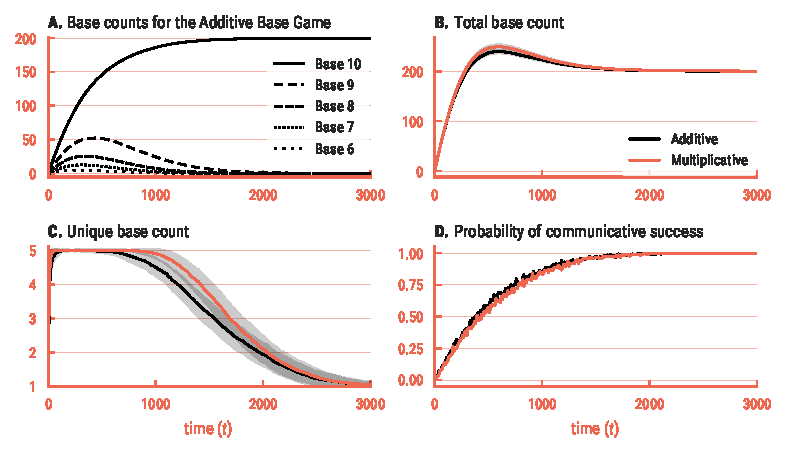
\includegraphics[trim=\figleftmarginA{} 0 0 \figtopmargin]{HUR03-results}	
	\caption{Comparison between the Additive Base Game (black) and the Multiplicative Base Game (orange). 
		The dynamics of the two games are remarkably similar.
		Dynamics are visualized using
		\subfig{A} the base counts of all possible bases for the Additive Base Game only (the Multiplicative case looks extremely similar);
		\subfig{B} the total base counts;
		\subfig{C} the unique base count; and
		\subfig{D} the probability of successful communication.
		See main text for details.
		\figdetails{\figid{hur03}
		Results shown for $N=200$, $B=10$, $\xi=1$; avg.\ of 600 runs; 1 std.\ shaded.
		}
		\label{fig:HUR03-results}}
\end{SCfigure}
%- - - - - - - -



%——————————————————————————————————————————————————————————
\paragraph{Basic Phenomenology}

Unlike \textcite{Hurford1987}, we have twenty years of agent-based modelling research at our disposal. 
I therefore reanalyse the games using a more modern methodology and analyse the following statistics
\begin{itemize}
	\item \textbf{(Probability of) communicative success $p_s(t)$} We consider an interaction successful if the base used by the speaker is favoured by the hearer. 
	\item \textbf{Base count $N_{\text{base}}(b, t)$.} 
		The number of agents that favour base $b$ at time $t$.
	\item \textbf{Total base count $N_{\text{total}}(t)$.} 
		The total number of bases favoured by agents in the population, i.e.
		$N_{\text{total}}(t) = \sum_b N_{\text{base}}(b, t)$.
	\item \textbf{Unique base count $N_{\text{unique}}(t)$.} The number of unique bases favoured in the population at time $t$, i.e.\ $N_{\text{unique}}(t) = |\{b: N_{\text{base}}(b, t) > 0\}|$.
\end{itemize}





Figure \ref{fig:HUR03-results} summarises the dynamics of the base games.
Subfigure \textsc{a} illustrates the typical stages every simulation goes through.
Initially, none of the bases is favoured and bases are used with roughly equal probability.
This is followed by a phase in which different bases compete for a share of the population.
The largest two bases are the two biggest competitors, but base 10 soon takes over, leading to the emergence of a shared, decimal system.
Subfigure \textsc{b} shows that multiple bases compete directly for each agent’s preference. 
This can be seen from the peak of $N_{\text{total}}$, which crosses the population size $N=200$, indicating that agents at that point on average favour more than one base.
Even when base 10 is already dominant, it can take a long time to eliminate all other bases from the population, as seen from \textsc{c}.
But in \textsc{d} one sees that population eventually communicates sucessfully.
The difference between the additive and multiplicative game, in terms of dynamics, appears to be small.
Most importantly, Hurford’s intuition about the emergence of a decimal system, is confirmed.





%——————————————————————————————————————————————————————————
%——————————————————————————————————————————————————————————
\section{Domain adaptivity in the base games}
%——————————————————————————————————————————————————————————
%——————————————————————————————————————————————————————————


The similarities between the dynamics of the base games (figure \ref{fig:HUR03-results}) and the dynamics of the naming games (e.g.~figure \ref{fig:LING01-strategies}) are striking.
Indeed, the base games seem to be naming games in disguise.
Rather than negotiating a name for an object, agents negotiate a base: which of the ‘words’ $6, \dots, 10$ should name the ‘object’ \textsc{base}.
Like the Bayesian language game, the ‘vocabulary’ is fixed to $K=5$ bases, and the strategy used corresponds directly to the \emph{frequency strategy} (when $\xi=1$). 





But there are also some striking dissimilarities.
Most notably, the same ‘word’ — base 10 — is adopted in every simulation:
The base game seems to be biased towards adopting the highest base. 
Hurford recognises this, but does not explain what this implicit bias exactly is.
But this can be done, for the additive base game, at least.
It is a nice mathematical puzzle to show that the probability that a base will be used (by an agent with no past experience) is
%-
\begin{align}
	\label{eq:ch6:bias-additive-naming-game}
	%-----
	p(b_j) 
		= \frac{1}{K} \bigl(H_K - H_{K-j}\bigr),
\end{align}
%-
where $H_n = \nicefrac{1}{1} + \dots + \nicefrac{1}{n}$ is the $n$’th harmonic number (see appendix \ref{app:counting-games} for a proof).
The distribution is plotted in figure \ref{fig:FIG10-base-game-bias.pdf}, for $B=10, 30$ and $60$.
The figure clearly demonstrates that the additive base game has a strong \emph{implicit bias} towards using the largest base.



\paragraph{Implicit biases and external constraints}


I have called the bias \emph{implicit} since the bias seems to be the result of certain constraints built into the model.
In this case, the constraints are arithmetic in nature and ensure that base 10 is much more expressive than base 6.
The constraints moreover appear to be \emph{external} to the agent — properties of the domain, rather than properties of the agent.\footnote{%
	%>>>
	Readers objecting to mathematical constraints being somehow external to the agents should note that this does not undermine the main point that biasses can differ in kind.
	%<<<
	}
This raises the question whether the \emph{implicit biases} arising from external constraints (“$13 > 6+6$”) should be distinguished from the biases somehow internal to the agent (“I have ten fingers”).
If the different biases influence the behaviour in qualitatively different ways, that is a clear indication that the two should be distinguished.
The next experiment shows that this is indeed the case.
%%




%- - - - - - - -
\begin{SCfigure}
	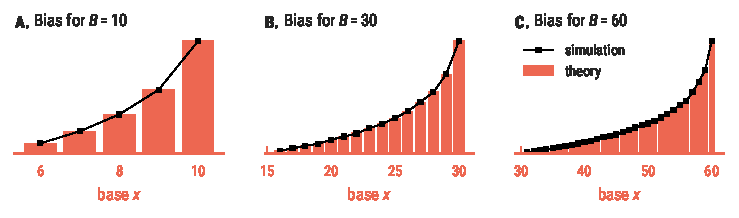
\includegraphics[trim=\figleftmarginA{} 0 0 \figtopmargin]{FIG10-base-game-bias}	
	
	\caption{%
	In the additive base game, the probability of using a base without any past experience (i.e., no preferences) is strongly skewed towards the highest base.
	The game has a strong implicit prior for using high bases.
	%----------
	\figdetails{\figid{fig10}
	The ‘simulation’ is the rel. freq. of 100 000 samples.}
	\label{fig:FIG10-base-game-bias.pdf}}
\end{SCfigure}
%- - - - - - - -




%- - - - - - - -
\begin{SCfigure}
	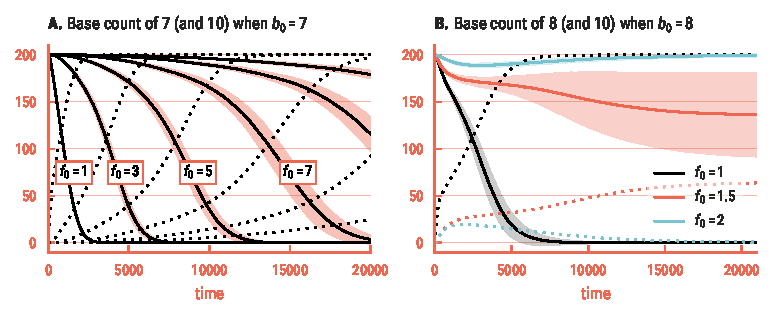
\includegraphics[trim=\figleftmarginA{} 0 0 \figtopmargin]{HUR05-results}	
	
	\caption{%
	The additive base game in populations biased towards using base 7 (left) or base 8 (right), with varying initial score $s_0$ (higher scores indicate stronger bias).
	The figure illustrates that the biases implicit in the domain and the biases of the agents work differently: agents cannot overcome the former (see main text for details).
	Note: averages over 300 runs are shown and for $s_0=1.5$ individual runs convert to either base 10 or base 8.
	%----------
	\figdetails{\figid{hur05}
		Results shown for $N=200$, $\eta=1$, $n_{\text{max}}=46$; avg.\ of 300 runs, 1 std.\ shaded.}
	\label{fig:effect-initial-conditions}}
\end{SCfigure}
%- - - - - - - -




Consider a population where every agent has an internal bias towards using a certain base. 
For example base 10, because the ten fingers are particularly salient. 
We model this by initially assigning a score $s_0$ to one particular base $b_0$.
These initial scores act as pseudo-observations, in the same way as the biases work in the Bayesian language game.
Figure \ref{fig:effect-initial-conditions}\textsc{a} reports an experiment with the additive base game where the population is biased towards using base $w_0 = 7$, with various different initial frequencies $s_0$.
The initial state seems to be unstable, irrespective of the initial frequency of base 7 (although it takes longer before base 7 dies out if the initial frequency is higher).
Apparently, a septenary system cannot be maintained. 
I presume this is so because base 7 can express only less than half of the numbers in the domain.
The probability that an agent will use another, larger base is therefore greater than the probability that it will use base 7, independent of whether it favours base 7.
This makes a septenary language unstable, and a larger base will eventually take over.
The important point is that the biases of the agents \emph{cannot overcome the  constraints of the domain}.
No matter how strong their initial bias for using base 7, nothing will change the fact that $7+7 < 15$, and the population will have to \emph{adapt} to the constraints in the domain.
%%




But the the internal biases and external constraints can interact in nontrivial ways.
Figure \ref{fig:effect-initial-conditions}\textsc{b} shows the same experiment, but now for a population biased towards base 8.
The behaviour is remarkably different. 
Most notably, an octal system \emph{can} be maintained, presumably since base 8 \emph{does} express more than half the numbers in the domain.
As a result, agents favouring base 8 are also more likely to use it.
But there is a caveat: the initial frequency must be large enough. 
If $s_0 \ge 2$, the population always adopts a base-8 system.
For $s_0 \le 1$, base-8 slowly dies out and the decimal system takes over.
But in between, $1 <s_0 < 2$ we observe a bifurcation. 
It should be noted that the plot shows the average over 300 runs.
In every such run, the population seems to adopt \emph{either} a decimal \emph{or} an octal system.
%%





These experiments demonstrate that the additive base game is not just the Bayesian naming game with a particular choice of bias.
This initially seems plausible, since the implicit biases takes the form of a distribution over $K$ bases $b_1, \dots, b_K$ and even the strategy ($\xi=1$) corresponds directly to a \textsc{map--map} strategy ($\eta=\zeta=\infty$) in the Dirichlet-categorical \textsc{ng}.
But since biases in that game act as pseudo-counts, sufficient counter-evidence will make the bias disappear.
Biases and experience are, in that respect, on completely equal footing.
In the additive base game, this is not the case. 
No amount of counter-evidence can overcome the external constraints in the sense that they never disappear.
We return to this point in the discussion.




%——————————————————————————————————————————————————————————
\paragraph{Domain adaptivity in the multiplicative base game}

The driving force behind the implicit bias in the additive base game is the difference in \emph{expressivity} between bases, with the largest base having a strong expressive advantage over the other bases.
One might wonder: are there other implicit biases, that come to the fore when bases are \emph{equally expressive}?
This is best studied in the multiplicative base game, which allows for larger domains.
The idea is to restrict the the domain such that no base has an expressive advantage. 
On a domain with upper bound $n_{\text{max}} = 6^2 + 10$, the limit of a multiplicative base-6 system, all all bases have equal expressivity.
If there are no other biases, the probability that base is adopted should be equal for all bases.
But initial experiments suggested that something very different was happening: the probability that a base would be adopted, depends on the size of the domain, i.e.\ on $n_{\text{max}}$.
The following experiment therefore takes a more general approach.
For every $n_{\text{max}} \in \{11, \dots, 110\}$, 600 simulations of 5000 iterations were repeated, with domain $I(n_{\text{max}}) = \{11, \dots, n_{\text{max}}\}$.\footnote{%
	%>>>
	In Hurford’s game, agents communicate about $\{21, \dots, 110\}$, but for this experiment the domain was extended.
	%<<<
	}
In each simulation, one particular base might be adopted.
The experiment aims to quantify the probability that a base is adopted on a certain domain, by averaging over 600 runs.\footnote{%
	%>>>
	More precisely, we recorded the final distribution over bases, since it sometimes happened that the population had not yet converged after 5000 iterations.
	%<<<
	}
I will call the distribution over adopted bases the \emph{distribution over outcomes}.
%%




%- - - - - - -
\begin{SCfigure}
	% Results HUR05
	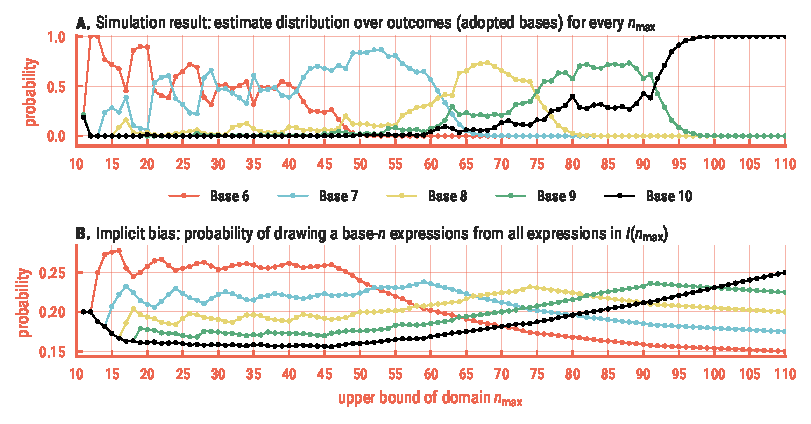
\includegraphics[trim=1.27cm 0 0 \figtopmargin]{HUR07-results}	
	\caption{Domain adaptivity in the multiplicative base game. 
		Figure \subfig{A} shows the distribution over outcomes (adopted bases) for every the domain $I(n_{\text{max}}) = \{11, \dots, n_{\text{max}}\}$.
		Note that the plot shows 99 distributions, one for each $n_{\text{max}}$.
		The game appears to exaggerate certain biases implicit in the domain. 
		Figure \subfig{B} shows an approximation of these biases: the probability that an expression randomly drawn from all expressions for numbers in $I(n_{\text{max}})$ uses base $b$.
		Details are in the main text.
		%----------
		\figdetails{
			\figid{hur07}
			Results shown for $N=200$, $\eta=1$. Each of the 99 distributions is the average over 600 runs.
			\label{fig:HUR07-results}
		}}
\end{SCfigure}
%- - - - - - -




Figure \ref{fig:HUR07-results}\textsc{a} shows the results.
Every  point on the $x$-axis corresponds to a domain $I(n_{\text{max}})$.
\emph{Above} that point, the distribution over outcomes is plotted.
The figure thus shows $110-11=99$ distributions.
It indicates that different bases are more likely to be adopted on different domains $I(n_{\text{max}})$.
When agents communicate about $I(18)$, base $6$ is adopted most frequently, when communicating about $I(70)$, base $8$ is most likely to emerge, etc.
The pattern is somewhat jumpy, but probably not because of random noise.
The estimates seem to be reliable, since averaging only 150 runs yields a similar pattern as the averages of 600 runs shown here.
There seems to be a \emph{structural} reason for the jumpiness, a bias implicit in the structure of the domain, to which the language adapts.
%%





In the additive base game, we specified the bias explicitly.
In this case, we will approximate it with the relative frequency of base-$b$ expressions.
How many ways there are to express a number $n$ using base $b$?
Consider $n=26$ and $b=6$.
The only possible expressions in the multiplicative base game are $4 \times 6 +2$ and $3\times 6 + 8$. 
More generally, the only two possible base $b$-expressions are:
%-
\begin{equation}
	\label{eq:ch6:base-b-expressions}
	%-----
	a\times b + c 
	\quad \text{and} \quad 
	(a-1) \times b + (b+c).
\end{equation}
%-
After all, for any lower factor $a-2$, the remainder would be at least $b+b+c > 2b > B$, and therefore inexpressible in the game.
So how many base-$b$ expressions does a number $n$ have? 
We denote this quantity by $N_b(n)$.
If $n > b^2+B$, it simply cannot be expressed and $N_b(n) = 0$.
Now let $c := n \text{ mod } b$. 
If $b+c > B$ then \eqref{eq:ch6:base-b-expressions} shows that $N_n(b)$ must be 1.
The same holds when $c = 0$, since preference is then given to the the simpler $x\times b + 0$.
In all other cases, there are 2 expressions, so in sum,
%-
\begin{align}
	N_b(n) = \begin{cases}
		0 	&\text{if $n> b^2 + B$}
		\\
		1	&\text{if $b+c > B$ or if $c=0$}
		\\
		2	&\text{otherwise}.
	\end{cases},
	\qquad c := n \text{ mod } b
\end{align}
%-
The total number of base-$b$ expressions for numbers in the interval $I(n_{\text{max}})$ is the sum $N_b(I(n_{\text{max}})) := \sum_{n=n_{\text{min}}}^{n_{\text{max}}} N_b(n)$,
and the relative frequency of base-$b$ expressions amongst all expressions in the interval $I(n_{\text{max}})$ is
%-
\begin{equation}
	f(b, n_{\text{max}}) := \frac{N_b(\; I(n_{\text{max}}) \;)}%
			{\sum_{b'} N_{b'}(\; I(n_{\text{max}}) \;)}.
\end{equation}
%-


Figure \ref{fig:HUR07-results}\textsc{b} shows the relative frequencies for all bases and 99 values of $n_{\text{max}}$, corresponding to subfigure  \textsc{a}.
The figure suggests that the relative frequency $f(b, n_{\text{max}})$ is a good first approximation of the implicit bias implicit in the domain, and the multiplicative base game seems to have exaggerated this bias.
The match is far from perfect, since we have not accounted for all complexities of the game.
First, the peaks in the implicit bias (subfigure \textsc{b}) have shifted to the left in the simulation results (subfigure \textsc{a}).
Consider the implicit bias towards base 6 in $I(90)$.
In an actual game with this domain, the base would never be adopted, since more than half of that domain is not expressible by base 6.
We have not accounted for that, but the game, of course, does and accordingly ‘shifts’ the implicit bias to the left (e.g.~6 has lower probability there).
Second, the game seems to exaggerate the implicit bias in the sense that bases with very low relative frequency are never adopted, and most probability mass is moved to the most frequent base.
This is in line with earlier findings about frequency strategies in chapter \ref{ch:bayesian-naming-games}, but does not seem to correspond to exponentiation alone.





Even though the approximation of the implicit biases is far from perfect, the experiment strongly suggests that there can be are other biases at play, besides the expressive advantage.
In this case the sheer number of expressions for a given number appears to give rise to a complex bias that makes different bases more likely to be adopted on different domains.
The language, numeral system, in this sense exhibits a kind of \emph{domain adaptivity}. 
The cultural process moreover seems to exaggerate the structure of the implicit bias, and the underlying reason might be the amplifying character of the frequency strategy.
In the final section of this chapter we further discuss the implicit biases.


%——————————————————————————————————————————————————————————
%——————————————————————————————————————————————————————————
\section{Counting games}
%——————————————————————————————————————————————————————————
%——————————————————————————————————————————————————————————


Hurford’s models only addressed the standardisation of a base and assumed that (1) the atoms of the system were in place and (2) that the additive or multiplicative constructions had been invented.
These two assumptions roughly correspond to the first three stages in the evolution of numeral systems as outlined in the previous chapter.
In this section, rather than assuming these stages, we attempt to reproduce them.
The first stage, the emergence of the first simple numerals, seems to be the type of problem naming games excel at.
The lowest numbers subitised and could therefore be named directly.
So, let’s suppose there is no homonymy, and agents need to negotiate, say, 3 numbers.
We could run the simulation, but there is really no need to do so: we already know that this works.
Playing a naming game with 3 objects in the absence of homonymy is the same as playing 3 independent single-object games at the same time (see figure \ref{fig:multi-word-minimal-naming-game}).



%%- - - - - - -
\begin{SCfigure}
	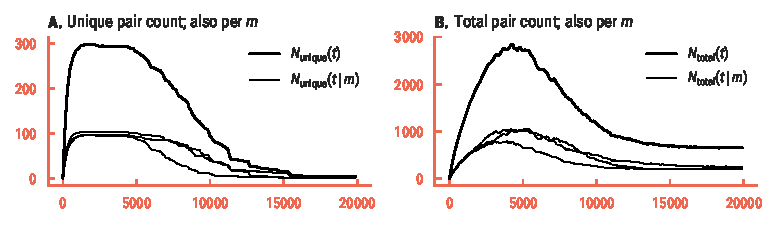
\includegraphics[trim=1.26cm 0 0 \figtopmargin]{FIG07-mw-naming-game}

	\caption{%
	A naming game with three objects is just the sum of three independent single-word \textsc{ng}’s when there is no homonymy.
	Dashed lines show the statistics per object; solid lines for the ‘total’ game: the sum of the dashed lines.
	%----------
	\figdetails{\figid{fig07}
	Results shown for 1 run; $N=200$, using the current strategy.}
	\label{fig:multi-word-minimal-naming-game}}
\end{SCfigure}
%%- - - - - - -



Can we extend this approach to the next stage, where a larger counting sequence of simple numerals emerges, by simply asking agents to negotiate more words?
Yes, but it raises a problem: nothing about the words signals that they are ordered (although their semantics of course does).
In fact, using a naming game to model the emergence of simple numerals commits to a certain conception of number.
Recall from the previous chapter that the \emph{referential-pragmatic hypothesis} holds that quantity is directly perceptible and can therefore be named unproblematically, as in a naming game.
For the lowest numbers up to around 4 this might be realistic, but for larger numerals, it is not.
The game we develop for that reason aims to align more closely with the \emph{ritual hypothesis} (and Hurford’s synthesis).
It assumes that numerals are grounded in a practice of counting \parencite{Hurford2007}: reciting a the sequence \lng{one, two, three}, and so on. 
As discussed in the previous chapter, this sequence might initially be a sequence of for example body parts.
The result is that the word \emph{eight} does not mean 8 because it refers to some object \textsc{eight}, but because it is the 8th word in a conventionalised counting sequence.
In this case, the semantics of numerals in a counting sequence are implicitly defined by their position in the sequence, by their order.
This implies that numerals are \emph{necessarily} ordered and continuous (uninterrupted), as some argue they should be \parencite{VonMengden2008}.




The goal then is to adapt the naming game so that agents negotiate a counting sequence.
To do so, first consider a naming game \emph{with} homonymy.  
In that case agents communicate object--word pairs $(o,w)$ where the same word can occur in different pairs.
For the population to reach coherence, the alignment strategy has to dampen competing pairs: all pairs using the same object, but a different word, \emph{or the same word, but a different object}.
All this is very similar to the original naming game, when words are replaced by pairs and the inhibition rules is extended accordingly.
We will use\footnote{%
	%>>>
	This is actually an unfortunate choice, since figure \ref{fig:LING01-strategies} suggests convergence is relatively slow.
	When doing this work, I was however not aware of the existence of lateral inhibition strategies and the like.
	%<<<
} lateral inhibition strategy 1 from \ref{table:li-strategies}, that is, with
%-
\begin{equation}
	\delta_{\text{inc}} 
		= \delta_{\text{inh}} 
		= \delta_{\text{init}} 
		= 1,
	\qquad
	\delta_{\text{dec}} = 0
\end{equation}
%-
Next, we replace object-word pairs by pairs of consecutive numerals: $(\text{one}, \text{two}), (\text{two}, \text{three})$, and so on. 
To illustrate this, suppose an agent knows the following pairs:
%-
\begin{align*}
	(\textsc{start}, \text{one}), 
	(\textsc{start}, \text{two}), 
	(\text{two}, \text{three}),
	(\text{two}, \text{four}),
	(\text{one}, \text{two}),
\end{align*}
%-
where \textsc{start} is a purely administrative symbol indicating the start of the counting sequence. The agent can form the following sequences:
%-
\begin{align*}
	&\text{\textsc{start}, one, two, three},
	&&\text{\textsc{start}, one, two, four},\\
	&\text{\textsc{start}, two, three},
	&&\text{\textsc{start}, two, four}
\end{align*}
%-
Other agents might be able to form different sequences, but the idea is that after many interactions, a consensus will emerge where only one sequence remains in use.
%%





In every interaction the agents must somehow communicate a \emph{sequence} of words, rather than single words.
This can be done in various ways, and I experimented with three slightly different scripts ($L$ denotes the \emph{limit} of the system):
%...
\begin{enumerate}
	\item \textbf{Unbounded counting game.}
	Starting from $x_0 = \textsc{start}$, the speaker iteratively chooses the next pair $(x_i, x_{i+1})$ with the highest score, \emph{generating as many new pairs as necessary}, until it reaches a randomly drawn number $n\le L$. 
	The sequence $(\textsc{start}, x_1, x_2, \dots, x_L)$ is presented to the hearer, who updates the score of every pair $(x_i, x_{i+1})$ according to the alignment strategy.
	(With $L=1$ this is a normal naming game.)

	\item \textbf{Instructional counting game.} 
	Similar to the unbounded version, but now the speaker can invent at most 1 new pair, \emph{whose score remains 0}, and always tries to count up to $L$ (rather than to $n \le L$). 
	In this game, agents can therefore only acquire new numerals if another agent instructed them how to count on.
	
	
	\item \textbf{Joint counting game.}
	Starting with \textsc{start}, the speaker utters the first word. 
	Both agents perform the usual updates.
	\emph{Only if the hearer knows the word}, i.e.\ if communication was successful, they continue with the next word.
	The round goes on in this fashion until communication breaks down or they reach $L$.
\end{enumerate}
%...
%%

To measure the dynamics of these games, besides the usual statistics the \emph{(counting sequence) length} $\ell(t)$ is measured: the length of the initial segment of the counting sequence about which the entire population agrees at time $t$.
It should also be noted that a complication arises when pairs are removed.
If one thinks of the pairs as describing a tree with \textsc{start} at the root, the removal of a pair can render an entire branch inaccessible.
To keep statistics like $N_{\text{total}}$ (which now counts pairs) informative, all inaccessible pairs are removed before collecting the statistics.
Finally, the communicative success is no longer boolean but averaged over all words in a round.



%- - - - - - - -
\begin{SCfigure}
	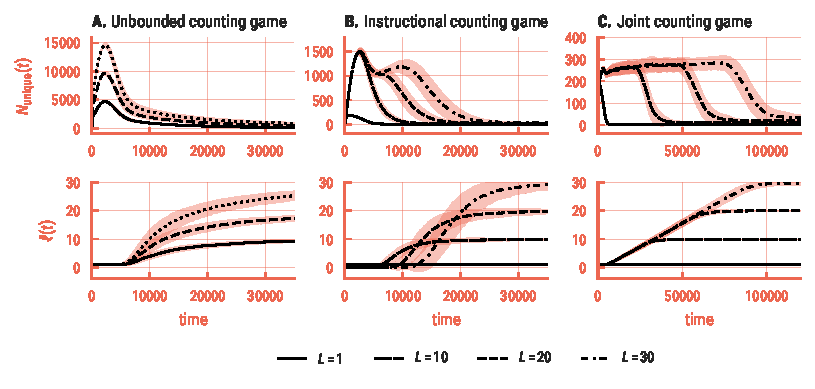
\includegraphics[trim=1.57cm 0 0 \figtopmargin]{counting-games}
	
	\caption{%
	Dynamics of the three counting games measured by the number of unique pairs and the initial segment length. 
	In all cases the population develops a counting sequence, but the dynamics are strikingly different. See main text for details.
	%----------
	\figdetails{Results shown for $N=200$; avg.\ of 600 runs, 1 std.\ shaded.}
	\label{fig:counting-games}}
\end{SCfigure}
%- - - - - - - 


The dynamics of the three games is visualised in figure \ref{fig:counting-games}.
All three games allow the population to negotiate a shared counting sequence, but in quite different ways.
In the unbounded counting game (\textsc{a}) convergence time does not depend on the limit $L$: negotiating 10, 20 or 30 simple numerals takes equally long.
Closer inspection reveals that the population has ‘found’ a simple trick.
My implementation happens to represent words by successive integers (rather than, say,  strings). 
A typical\footnote{%
	%>>>
	I have checked all this by computing the distribution of fragment lengths for every $L$.
	%<<<
	} counting sequence at the end of the game turns out to be of the form
\[
	\textsc{start}, \;
	\underbrace{212, 213, 214}_{\text{fragment 1}}, \; 
	\underbrace{350, 351, 352, 353}_{\text{fragment 2}}, \;
	\underbrace{658, 659, 660}_{\text{fragment 3}}.
\]
where the numbers are ‘words’ and every fragment is generated by a single speaker. 
It seems that the population has ‘adapted’ to a higher $L$ by communicating \emph{fragments} rather than pairs.
Since fragments become larger when $L$ does, convergence times remain approximately stable. 



In the instructional game this cannot happen, since in every encounter at most one word can be invented.
But the game does exhibit some funny behaviour.
If a population for example has to count up to $L=10$, they can do so earlier than when they have to count up to $L=30$. This can be seen from the length $\ell(t)$ in figure \ref{fig:counting-games}\textsc{b} and is, of course, mildly absurd.
Interestingly, the joint counting game results in perfectly linear behaviour: the population is always exactly on the same page.
After all, a speaker can only count on if the hearer agreed about the sequence so far.



\paragraph{Simple numerals, and beyond?}

Populations of counting agents can negotiate a counting sequence, so can they go on and negotiate a recursive numeral system?
The idea was again to again take inspiration from the evolutionary account in chapter \ref{ch:numerals} and see if a practice of ‘grouping’ could give rise to serialisation, or, simply put, additive constructions: ten stones and another 3 \parencite{Hurford2007}.
When counting agents could at some point decide to group what they had counted so far. 
This means that agents have to score possible group sizes — bases, really — and use a base depending on its score.
In other words, agents would have to play a naming game to negotiate the group size, the base, while simultaneously playing a counting game to negotiate a sequence of atoms.
These two problems are interdependent: the length of the counting sequence is determined by the base, or, conversely, the base is the numeral where the counting sequence of atoms ends.




What I typically observed in all experiments with games of this type — I considered many variations on this theme — was that negotiating a single base is much easier than negotiating a long counting sequence.
The population would thus adopt the first base it could count to (typically 2, as I excluded group size 1).
To prevent this from happening one should, in one way or another, get the population to postpone the negotiation of the base, until the counting sequence has developed sufficiently.
But this amounts to implementing an implicit bias towards a certain base.
I did not continue along these lines, since it appeared to add little to our understanding of the the evolution of numeral systems.
After all, if the model is in the end bringing some implicit biases to the fore, one might as well take the Bayesian naming game and encode the biases explicitly as a prior.







\section{Conclusions}

This chapter explored the first experiments trying to align agent-based simulations of the cultural evolution of numeral systems with their actual evolution, as discussed in chapter \ref{ch:numerals}.
The starting point was the pioneering work of James Hurford, who introduced the  base games where the population negotiated a shared base with additive and multiplicative constructions.
Detailed analyses suggested that the base games implements a strong implicit biases towards the highest base, resulting from the expressive advantage that base has: it can express all the numbers in the domain, whereas the smallest base can only express a few numbers.
When this advantages is removed by restricting the domain such that all bases have equal expressivity, more subtle frequency patterns in the domain appear to determine the outcome of the cultural process.
Further analyses revealed that the biases implicit in the domain affect the behaviour of the game differently than biases of agents.
The latter can be overcome by counter evidence, the former cannot.




The findings highlight one simple point: naming games can be driven by implicit biases.
This is reminiscent of early iterated learning models, where the biases leading to the emergence of compositionality were often hard to isolate.
In iterated learning literature \parencite{Kirby2007,Kirby2007} explicit biases are often advocated, as is done in Bayesian models.
The additive base game provide a compelling argument for doing the same with naming games.
Explicating the biases, as we did in \eqref{eq:ch6:bias-additive-naming-game}, makes transparent to what extend the outcome (a decimal system) is determined by the assumptions in the model.
However, we have also seen that hard constraints influence the behaviour of the model differently than the biases in for example the Bayesian naming games.
This suggests that Bayesian models not only introduced explicit biases in the iterated learning literature, but might also have changed the way the biases work compared to early iterated learning models.






Although the games exhibit a certain domain adaptivity, one must be careful not to jump to the conclusion that numeral systems are shaped by their domain.
After all, the adaptivity in the multiplicative base game is rather artificial.\footnote{%
	%>>>
	It might be interesting to note that in some trial experiments where, as the result of some bugs in the implementation, prime numbers had a slight frequency advantage, leading to the emergence of prime bases.
	Clearly these kind of biases are not driving the evolution of numeral systems.
	%<<<
	}
Base 6 has higher expressivity on, say, $I(18)$ than base 10, only because the game allows the summand $c$ in an expression $a \times b +c$ to be larger than the base $b$, as seen from \eqref{eq:ch6:base-b-expressions}.\footnote{%:
	%>>>
	I am not sure if \textcite{Hurford1987} was aware of this. His definition of a base is explicit and implies that “7 would be the the base in both $(3 \times 7)$ and $((4 \times 7) + 3)$” (p.~295). He also mentions expressions such as $3\times 4 + 9$ (p.~294), which leave me to conclude that he did not rule out overrunning.
	%<<<
	}
Such \emph{overrunning} is rarely found in actual numeral systems, as discussed in the previous chapter.
That adaptivity of the multiplicative base game (figure \ref{fig:HUR07-results}) is therefore an artefact of overrunning.
It further implies that synonymy only disappears if the domain is not restricted, that is, if base 10 \emph{does} have an expressive advantage.
On smaller domains a population might evolve a base 6 system, where both the expressions $3\times 6 + 8$ and $4 \times 6 + 2$ would be perfectly ‘standard’.
This is not only undesirable for a model of standardisation, it also has consequences for the packing strategy, which Hurford’s simulations partly aimed to explain.
The first of these expressions, after all, violates the packing strategy.




\paragraph{Mechanisms and interpretations}


Although the base games indicate that social processes can lead to standardisation of a base, that is not to say that the model is\emph{realistic}.
Roughly, the models suggest that standardisation arises because people prefer to use the most frequently observed bases.
Interestingly Hurford himself suggests a very different explanation before introducint his simulations, arguing that standardisation would arise because “the obvious communicative advantages of standardised, canonical forms, and because no communicative advantage is lost by such a standardisation, due to the rather special nature of numerals/numbers” (p.~273).
Something along those lines indeed seems plausible, but such explanations are not supported by the models.
I think this highlights a serious difficulty for the use of models: the mechanism and the interpretation need not be aligned.
That is, the mathematical explanation of why a model exhibits the behaviour it does, is often not in line with the interpretation given to the model, since that is typically based only on the behaviour observed in simulations.
And insofar the interpretation and the mechanism are misaligned, modelling does not contribute much to showing the consistency of an informal account either.
One way to resolve such discrepancies is by evaluating models against empirical data: by testing the underlying mechanisms and the predictions they make.


When it comes to that, the base games do not await a very bright future.
They for example predict that higher bases are more likely to be adopted, while in fact bases higher than 20 are rare \parencite{Hammarstrom2009}.
Moreover, numeral systems use multiple bases to counter expressive restrictions, so the disadvantage of a base-6 system in the base games is in reality ameliorated by introducing the larger base 36.


% Print the bibliography
\showbibliography


\end{document}


The biggest problem, however: compositionality results from a rather down to earth practice

Discussion: 
- bases appear in tandem with serialisation, not, as hurford described, after the emergence of additive constructions
